% !TEX TS-program = pdflatex
\documentclass[11pt]{article}

% -------------------- Packages --------------------
\usepackage[a4paper,margin=1in]{geometry}
\usepackage{amsmath,amssymb}
\usepackage[T1]{fontenc}
\usepackage{lmodern}
\usepackage{xcolor}
\usepackage{tcolorbox}
\tcbuselibrary{skins,breakable}
\usepackage{enumitem}
\usepackage{hyperref}
\usepackage{tikz}
\usetikzlibrary{calc,angles,quotes}

\pagestyle{empty}

% -------------------- Dark Theme Colors --------------------
\definecolor{bg}{HTML}{000000}
\definecolor{pairbg}{HTML}{121212}
\definecolor{solbg}{HTML}{0A0A0A}
\definecolor{border}{HTML}{2A2A2A}
\definecolor{text}{HTML}{FFFFFF}
\definecolor{muted}{HTML}{C9CDD3}
\definecolor{gold}{HTML}{FFD700}
\definecolor{green}{HTML}{4ADE80}
\definecolor{cyan}{HTML}{38BDF8}

\pagecolor{bg}
\color{text}

\hypersetup{
  colorlinks=true,
  linkcolor=cyan,
  urlcolor=cyan
}

\setlength{\parindent}{0pt}
\setlength{\parskip}{10pt}

\setlist[itemize]{left=1.4em,itemsep=6pt,topsep=6pt}
\setlist[enumerate]{left=1.6em,itemsep=4pt,topsep=4pt}

% -------------------- tcolorbox Base --------------------
\tcbset{
  enhanced,
  breakable,
  arc=12pt,
  boxrule=0.8pt,
  left=16pt,right=16pt,top=12pt,bottom=12pt
}

\newtcolorbox{QAPair}[1]{%
  colback=pairbg,
  colbacklower=solbg,
  colframe=border,
  coltext=text,
  title=\textcolor{gold}{\bfseries #1},
  fonttitle=\bfseries,
  coltitle=text,
  segmentation style={draw=border, dashed, line width=0.6pt},
}

% Visible text inside this box (fix)
\newtcolorbox{QuickBox}{%
  colback=pairbg,
  colframe=cyan,
  coltext=text,
  fontupper=\color{text},
  borderline north={4pt}{0pt}{cyan},
  arc=14pt,
  boxrule=0.8pt
}

% Helper for step headings
\newcommand{\Step}[1]{\textcolor{muted}{\textbf{Step #1:}}}

% ============================================================
\begin{document}

\begin{center}
{\LARGE\bfseries \textcolor{gold}{Exercise 9.5 --- Solutions}}\\[-2pt]
\end{center}

\begin{QuickBox}
{\color{cyan}\bfseries Quick formulas (Polygons)}\par\medskip
\begin{itemize}
\item \textbf{Sum of exterior angles (any convex polygon):} $\sum e = 360^\circ$.
\item \textbf{Regular $n$-gon:} each exterior angle $e=\dfrac{360^\circ}{n}$.
\item \textbf{Regular $n$-gon:} each interior angle $i=180^\circ-e=180^\circ-\dfrac{360^\circ}{n}$.
\item \textbf{Sum of interior angles:} $\sum i=(n-2)\cdot 180^\circ$.
\item \textbf{Interior + corresponding exterior:} $i+e=180^\circ$ (supplementary).
\item \textbf{Number of diagonals:} $D=\dfrac{n(n-3)}{2}$.
\end{itemize}
\end{QuickBox}

% ============================================================
% Q1
\begin{QAPair}{Question 1 (a)}
\textcolor{gold}{\bfseries Question:} Find the number of sides of a regular polygon if each exterior angle is $45^\circ$.\\
\tcblower
\textcolor{green}{\bfseries Answer:}
\[
\begin{aligned}
\Step{1}\;& e=\frac{360^\circ}{n}\\
\Step{2}\;& 45^\circ=\frac{360^\circ}{n}\ \Rightarrow\ n=\frac{360}{45}=8.
\end{aligned}
\]
\[
\boxed{n=8\ \text{(octagon)}}
\]
\end{QAPair}

\begin{QAPair}{Question 1 (b)}
\textcolor{gold}{\bfseries Question:} Find the number of sides of a regular polygon if each exterior angle is $60^\circ$.\\
\tcblower
\textcolor{green}{\bfseries Answer:}
\[
\begin{aligned}
\Step{1}\;& 60^\circ=\frac{360^\circ}{n}\\
\Step{2}\;& n=\frac{360}{60}=6.
\end{aligned}
\]
\[
\boxed{n=6\ \text{(hexagon)}}
\]
\end{QAPair}

\begin{QAPair}{Question 1 (c)}
\textcolor{gold}{\bfseries Question:} Find the number of sides of a regular polygon if each exterior angle is $120^\circ$.\\
\tcblower
\textcolor{green}{\bfseries Answer:}
\[
\begin{aligned}
\Step{1}\;& 120^\circ=\frac{360^\circ}{n}\\
\Step{2}\;& n=\frac{360}{120}=3.
\end{aligned}
\]
\[
\boxed{n=3\ \text{(triangle)}}
\]
\end{QAPair}

\begin{QAPair}{Question 1 (d)}
\textcolor{gold}{\bfseries Question:} Find the number of sides of a regular polygon if each exterior angle is $40^\circ$.\\
\tcblower
\textcolor{green}{\bfseries Answer:}
\[
\begin{aligned}
\Step{1}\;& 40^\circ=\frac{360^\circ}{n}\\
\Step{2}\;& n=\frac{360}{40}=9.
\end{aligned}
\]
\[
\boxed{n=9\ \text{(nonagon)}}
\]
\end{QAPair}

% ============================================================
% Q2
\begin{QAPair}{Question 2}
\textcolor{gold}{\bfseries Question:} Draw a regular pentagon whose exterior angles are $p,q,r,s,t$ and each interior angle is $k$. What is the measure of:\\
(a) each interior angle \quad (b) each exterior angle.\\
\tcblower
\textcolor{green}{\bfseries Answer:}

\textcolor{muted}{\textbf{Diagram (regular pentagon):}}
\[
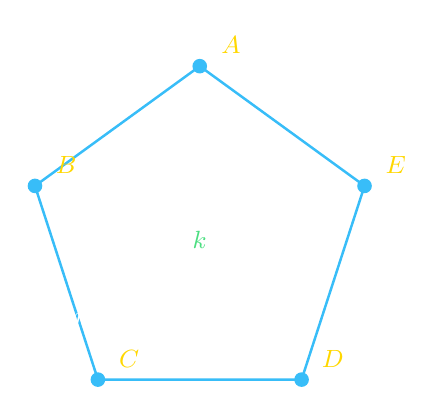
\begin{tikzpicture}[scale=2.2, every node/.style={color=text, font=\small}]
  \foreach \i [evaluate=\i as \ang using 90+72*\i] in {0,...,4}{
    \coordinate (P\i) at (\ang:1);
  }
  \draw[cyan, line width=0.9pt] (P0)--(P1)--(P2)--(P3)--(P4)--cycle;

  \foreach \i/\lab in {0/A,1/B,2/C,3/D,4/E}{
    \fill[cyan] (P\i) circle (1.2pt);
    \node[gold] at ($(P\i)+(0.18,0.12)$) {$\lab$};
  }

  % Labels for exterior angles near vertices (symbolic)
  \node at ($(P0)+(0.35,0.10)$) {$p$};
  \node at ($(P1)+(0.25,0.30)$) {$q$};
  \node at ($(P2)+(-0.10,0.35)$) {$r$};
  \node at ($(P3)+(-0.33,0.15)$) {$s$};
  \node at ($(P4)+(0.00,-0.35)$) {$t$};

  % Label interior angle k in the middle
  \node[green] at (0,0) {$k$};
\end{tikzpicture}
\]

\[
\begin{aligned}
\Step{1}\;& \text{For a regular }5\text{-gon, each exterior angle } e=\frac{360^\circ}{5}=72^\circ.\\
\Step{2}\;& \text{Each interior angle } k = 180^\circ - e = 180^\circ-72^\circ = 108^\circ.
\end{aligned}
\]

\[
\boxed{\text{(a) }k=108^\circ \qquad \text{(b) }p=q=r=s=t=72^\circ}
\]
\end{QAPair}

% ============================================================
% Q3
\begin{QAPair}{Question 3}
\textcolor{gold}{\bfseries Question:} Each interior angle of a polygon is five times the exterior angle of the polygon. Find the number of sides.\\
\tcblower
\textcolor{green}{\bfseries Answer:}
Let exterior angle be $e$. Then interior angle $i=5e$.
\[
\begin{aligned}
\Step{1}\;& i+e=180^\circ \Rightarrow 5e+e=180^\circ\\
\Step{2}\;& 6e=180^\circ \Rightarrow e=30^\circ\\
\Step{3}\;& e=\frac{360^\circ}{n} \Rightarrow 30^\circ=\frac{360^\circ}{n}\Rightarrow n=\frac{360}{30}=12.
\end{aligned}
\]
\[
\boxed{n=12\ \text{(dodecagon)}}
\]
\end{QAPair}

% ============================================================
% Q4
\begin{QAPair}{Question 4}
\textcolor{gold}{\bfseries Question:} Find the minimum interior angle and maximum exterior angle possible in a regular polygon. Give reasons.\\
\tcblower
\textcolor{green}{\bfseries Answer:}
For a regular $n$-gon ($n\ge 3$):
\[
e=\frac{360^\circ}{n},\qquad i=180^\circ-\frac{360^\circ}{n}.
\]

\[
\begin{aligned}
\Step{1}\;& e=\frac{360^\circ}{n}\ \text{is largest when }n\text{ is smallest.}\\
\Step{2}\;& \text{Smallest possible }n\text{ is }3\ (\text{triangle}).\\
\Step{3}\;& e_{\max}=\frac{360^\circ}{3}=120^\circ,\quad
i_{\min}=180^\circ-120^\circ=60^\circ.
\end{aligned}
\]
\[
\boxed{i_{\min}=60^\circ \text{ and } e_{\max}=120^\circ\ (\text{both for an equilateral triangle})}
\]
\end{QAPair}

% ============================================================
% Q5
\begin{QAPair}{Question 5 (a)}
\textcolor{gold}{\bfseries Question:} Find the exterior angle of a regular polygon of $5$ sides.\\
\tcblower
\textcolor{green}{\bfseries Answer:}
\[
e=\frac{360^\circ}{n}=\frac{360^\circ}{5}=72^\circ
\quad\Rightarrow\quad
\boxed{72^\circ}
\]
\end{QAPair}

\begin{QAPair}{Question 5 (b)}
\textcolor{gold}{\bfseries Question:} Find the exterior angle of a regular polygon of $9$ sides.\\
\tcblower
\textcolor{green}{\bfseries Answer:}
\[
e=\frac{360^\circ}{9}=40^\circ
\quad\Rightarrow\quad
\boxed{40^\circ}
\]
\end{QAPair}

\begin{QAPair}{Question 5 (c)}
\textcolor{gold}{\bfseries Question:} Find the exterior angle of a regular polygon of $15$ sides.\\
\tcblower
\textcolor{green}{\bfseries Answer:}
\[
e=\frac{360^\circ}{15}=24^\circ
\quad\Rightarrow\quad
\boxed{24^\circ}
\]
\end{QAPair}

\begin{QAPair}{Question 5 (d)}
\textcolor{gold}{\bfseries Question:} Find the exterior angle of a regular polygon of $20$ sides.\\
\tcblower
\textcolor{green}{\bfseries Answer:}
\[
e=\frac{360^\circ}{20}=18^\circ
\quad\Rightarrow\quad
\boxed{18^\circ}
\]
\end{QAPair}

% ============================================================
% Q6
\begin{QAPair}{Question 6}
\textcolor{gold}{\bfseries Question:} The ratio between an exterior angle and the interior angle of a regular polygon is $1:2$. Find:\\
(a) each exterior angle \quad (b) each interior angle \quad (c) number of sides.\\
\tcblower
\textcolor{green}{\bfseries Answer:}
Let exterior angle $e$ and interior angle $i$.
\[
\Step{1}\; \frac{e}{i}=\frac{1}{2}\Rightarrow i=2e.
\]
\[
\begin{aligned}
\Step{2}\;& i+e=180^\circ \Rightarrow 2e+e=180^\circ\\
\Step{3}\;& 3e=180^\circ \Rightarrow e=60^\circ\\
\Step{4}\;& i=2e=2(60^\circ)=120^\circ\\
\Step{5}\;& e=\frac{360^\circ}{n}\Rightarrow 60^\circ=\frac{360^\circ}{n}\Rightarrow n=\frac{360}{60}=6.
\end{aligned}
\]
\[
\boxed{\text{(a) }e=60^\circ\qquad \text{(b) }i=120^\circ\qquad \text{(c) }n=6}
\]
\end{QAPair}

% ============================================================
% Q7
\begin{QAPair}{Question 7}
\textcolor{gold}{\bfseries Question:} Is it possible to have a regular polygon each of whose exterior angle is $50^\circ$? Give reason.\\
\tcblower
\textcolor{green}{\bfseries Answer:}
For a regular polygon,
\[
e=\frac{360^\circ}{n}.
\]
If $e=50^\circ$, then
\[
n=\frac{360}{50}=7.2,
\]
but $n$ must be a whole number.
\[
\boxed{\text{Not possible, because } \frac{360}{50}\ \text{is not an integer.}}
\]
\end{QAPair}

% ============================================================
% Q8
\begin{QAPair}{Question 8}
\textcolor{gold}{\bfseries Question:} Name the polygon whose sum of interior angles is equal to the sum of its exterior angles.\\
\tcblower
\textcolor{green}{\bfseries Answer:}
\[
\begin{aligned}
\Step{1}\;& \sum \text{exterior}=360^\circ\\
\Step{2}\;& \sum \text{interior}=(n-2)\cdot 180^\circ\\
\Step{3}\;& (n-2)\cdot 180^\circ=360^\circ \Rightarrow n-2=2 \Rightarrow n=4.
\end{aligned}
\]
\[
\boxed{\text{Quadrilateral }(4\text{ sides})}
\]
\end{QAPair}

% ============================================================
% Q9
\begin{QAPair}{Question 9}
\textcolor{gold}{\bfseries Question:} The sum of all the interior angles of a regular polygon is four times the sum of its exterior angles. Identify the polygon.\\
\tcblower
\textcolor{green}{\bfseries Answer:}
\[
\begin{aligned}
\Step{1}\;& \sum \text{exterior}=360^\circ\\
\Step{2}\;& \sum \text{interior}=4\times 360^\circ=1440^\circ\\
\Step{3}\;& (n-2)\cdot 180^\circ=1440^\circ\\
\Step{4}\;& n-2=\frac{1440}{180}=8 \Rightarrow n=10.
\end{aligned}
\]
\[
\boxed{\text{Decagon }(10\text{ sides})}
\]
\end{QAPair}

% ============================================================
% Q10
\begin{QAPair}{Question 10}
\textcolor{gold}{\bfseries Question:} An exterior angle of a regular polygon is $12^\circ$. What is the sum of all the interior angles?\\
\tcblower
\textcolor{green}{\bfseries Answer:}
\[
\begin{aligned}
\Step{1}\;& e=\frac{360^\circ}{n}\Rightarrow 12^\circ=\frac{360^\circ}{n}\Rightarrow n=\frac{360}{12}=30.\\
\Step{2}\;& \sum \text{interior}=(n-2)\cdot 180^\circ=(30-2)\cdot 180^\circ=28\cdot 180^\circ.
\end{aligned}
\]
\[
28\cdot 180=28\cdot (100+80)=2800+2240=5040.
\]
\[
\boxed{\sum \text{interior}=5040^\circ}
\]
\end{QAPair}

% ============================================================
% Q11
\begin{QAPair}{Question 11}
\textcolor{gold}{\bfseries Question:} Prove that each interior angle and its corresponding exterior angle in any polygon are supplementary.\\
\tcblower
\textcolor{green}{\bfseries Answer:}

\textcolor{muted}{\textbf{Diagram (linear pair at a vertex):}}
\[
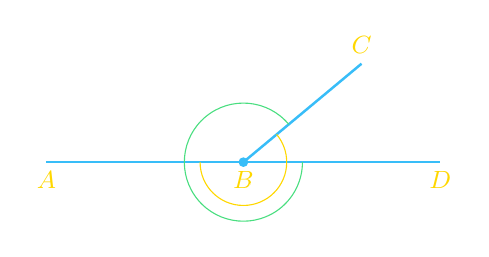
\begin{tikzpicture}[scale=1.25, every node/.style={color=text, font=\small}]
  \coordinate (A) at (-2,0);
  \coordinate (B) at (0,0);
  \coordinate (D) at (2,0);
  \coordinate (C) at (1.2,1);

  \draw[cyan, line width=0.9pt] (A)--(B)--(D);
  \draw[cyan, line width=0.9pt] (B)--(C);

  \fill[cyan] (B) circle (1.4pt);

  \node[gold] at (A) [below] {$A$};
  \node[gold] at (B) [below] {$B$};
  \node[gold] at (D) [below] {$D$};
  \node[gold] at (C) [above] {$C$};

  \pic[draw=gold, angle radius=0.55cm, "$i$"] {angle=A--B--C};
  \pic[draw=green, angle radius=0.75cm, "$e$"] {angle=C--B--D};
\end{tikzpicture}
\]

\[
\begin{aligned}
\Step{1}\;& \text{At vertex }B,\ \overline{AB}\text{ and }\overline{BD}\text{ are the same straight line.}\\
\Step{2}\;& \angle ABC\ \text{(interior)}=i,\ \angle CBD\ \text{(exterior)}=e.\\
\Step{3}\;& \angle ABC\ \text{and}\ \angle CBD\ \text{form a linear pair on a straight line.}\\
\Step{4}\;& \text{Angles on a straight line sum to }180^\circ.\\
\Step{5}\;& \Rightarrow\ i+e=180^\circ.
\end{aligned}
\]
\[
\boxed{\text{Hence, each interior angle and its corresponding exterior angle are supplementary.}}
\]
\end{QAPair}

% ============================================================
% Q12
\begin{QAPair}{Question 12}
\textcolor{gold}{\bfseries Question:} Find the number of sides in a regular polygon when the measure of each exterior angle is $72^\circ$.\\
\tcblower
\textcolor{green}{\bfseries Answer:}
\[
\begin{aligned}
\Step{1}\;& 72^\circ=\frac{360^\circ}{n}\\
\Step{2}\;& n=\frac{360}{72}=5.
\end{aligned}
\]
\[
\boxed{n=5\ \text{(pentagon)}}
\]
\end{QAPair}

% ============================================================
% Q13
\begin{QAPair}{Question 13}
\textcolor{gold}{\bfseries Question:} The exterior angles of a pentagon are $(y+5)^\circ$, $(2y+3)^\circ$, $(3y+2)^\circ$, $(4y+1)^\circ$, and $(5y+4)^\circ$. Find the measure of each angle.\\
\tcblower
\textcolor{green}{\bfseries Answer:}
\[
\Step{1}\; \text{Sum of exterior angles of any pentagon }=360^\circ.
\]
\[
\begin{aligned}
\Step{2}\;& (y+5)+(2y+3)+(3y+2)+(4y+1)+(5y+4)=360\\
\Step{3}\;& (1+2+3+4+5)y + (5+3+2+1+4)=360\\
\Step{4}\;& 15y+15=360 \Rightarrow 15y=345 \Rightarrow y=\frac{345}{15}=23.
\end{aligned}
\]
Now substitute $y=23$:
\[
\boxed{
\begin{aligned}
(y+5)^\circ&=(23+5)^\circ=28^\circ\\
(2y+3)^\circ&=(46+3)^\circ=49^\circ\\
(3y+2)^\circ&=(69+2)^\circ=71^\circ\\
(4y+1)^\circ&=(92+1)^\circ=93^\circ\\
(5y+4)^\circ&=(115+4)^\circ=119^\circ
\end{aligned}}
\]
\end{QAPair}

% ============================================================
% Q14
\begin{QAPair}{Question 14}
\textcolor{gold}{\bfseries Question:} A convex polygon has $14$ diagonals. Find the number of sides of the polygon.\\
\tcblower
\textcolor{green}{\bfseries Answer:}
\[
\begin{aligned}
\Step{1}\;& D=\frac{n(n-3)}{2}\\
\Step{2}\;& 14=\frac{n(n-3)}{2}\Rightarrow 28=n(n-3)\\
\Step{3}\;& n^2-3n-28=0\\
\Step{4}\;& (n-7)(n+4)=0 \Rightarrow n=7\ (\text{positive solution}).
\end{aligned}
\]
\[
\boxed{n=7\ \text{(heptagon)}}
\]
\end{QAPair}

% ============================================================
% Q15
\begin{QAPair}{Question 15}
\textcolor{gold}{\bfseries Question:} Find the sum of all the interior angles of a polygon having $13$ sides.\\
\tcblower
\textcolor{green}{\bfseries Answer:}
\[
\begin{aligned}
\Step{1}\;& \sum \text{interior}=(n-2)\cdot 180^\circ\\
\Step{2}\;& =(13-2)\cdot 180^\circ=11\cdot 180^\circ=1980^\circ.
\end{aligned}
\]
\[
\boxed{1980^\circ}
\]
\end{QAPair}

% ============================================================
% Q16
\begin{QAPair}{Question 16}
\textcolor{gold}{\bfseries Question:} The sum of all the interior angles of a polygon is $2880^\circ$. How many sides does the polygon have?\\
\tcblower
\textcolor{green}{\bfseries Answer:}
\[
\begin{aligned}
\Step{1}\;& (n-2)\cdot 180^\circ=2880^\circ\\
\Step{2}\;& n-2=\frac{2880}{180}=16\\
\Step{3}\;& n=18.
\end{aligned}
\]
\[
\boxed{n=18\ \text{(18-gon)}}
\]
\end{QAPair}

\end{document}
